\documentclass[tikz,border=2pt]{standalone}
\usepackage{amsmath,amssymb}
\usepackage{tikz}
\usetikzlibrary{arrows.meta}

\begin{document}
% Sandwiching the unknown optimum of a maximisation problem: any feasible (heuristic)
% solution gives a lower bound z_H, any relaxation an upper bound z_R; the gap bounds the error.
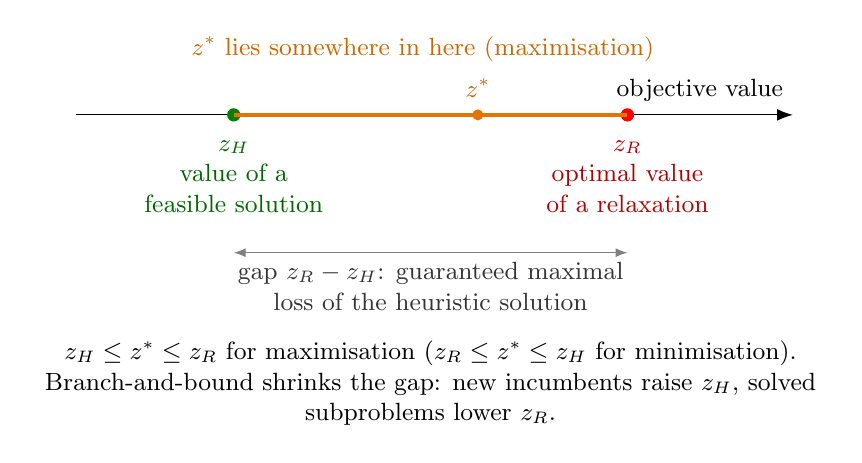
\begin{tikzpicture}[every node/.style={font=\small}, >={Latex[length=2mm]}]
	\draw[->] (-0.5,0) -- (8.6,0);
	\node[anchor=south east] at (8.6,0.05) {objective value};
	\fill[green!50!black] (1.5,0) circle (2.4pt);
	\node[green!40!black, anchor=north, align=center] at (1.5,-0.2) {$z_H$\\ value of a\\ feasible solution};
	\fill[red] (6.5,0) circle (2.4pt);
	\node[red!70!black, anchor=north, align=center] at (6.5,-0.2) {$z_R$\\ optimal value\\ of a relaxation};
	\draw[orange!90!black, very thick] (1.5,0) -- (6.5,0);
	\node[orange!80!black, anchor=south] at (3.9,0.55) {$z^\ast$ lies somewhere in here (maximisation)};
	\fill[orange!90!black] (4.6,0) circle (2pt);
	\node[orange!80!black, anchor=south] at (4.6,0.1) {$z^\ast$};
	\draw[{Latex[length=1.5mm]}-{Latex[length=1.5mm]}, gray] (1.5,-1.75) -- (6.5,-1.75) node[midway, below, align=center, text=gray!40!black] {gap $z_R-z_H$: guaranteed maximal\\ loss of the heuristic solution};
	\node[anchor=north, align=flush center, text width=10cm] at (4.0,-2.75) {$z_H\le z^\ast\le z_R$ for maximisation ($z_R\le z^\ast\le z_H$ for minimisation). Branch-and-bound shrinks the gap: new incumbents raise $z_H$, solved subproblems lower $z_R$.};
\end{tikzpicture}
\end{document}
